

\tikzset{every picture/.style={line width=0.75pt}} %set default line width to 0.75pt        

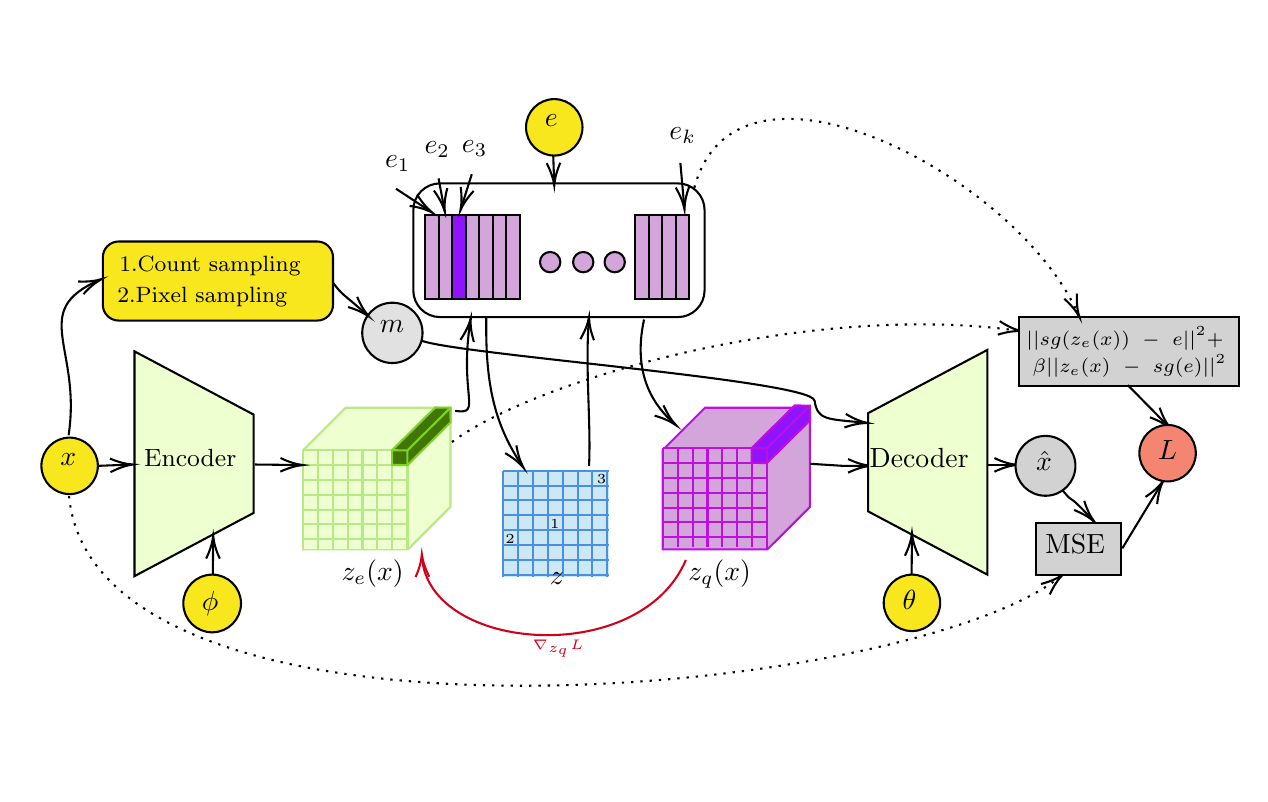
\begin{tikzpicture}[x=0.75pt,y=0.75pt,yscale=-1,xscale=1]
%uncomment if require: \path (0,308); %set diagram left start at 0, and has height of 308

%Shape: Trapezoid [id:dp6171005453979647] 
\draw  [fill={rgb, 255:red, 238; green, 255; blue, 208 }  ,fill opacity=1 ] (107.75,142.44) -- (165.17,172.91) -- (165.17,220.26) -- (107.75,250.73) -- cycle ;
%Shape: Cube [id:dp24555481618180852] 
\draw  [color={rgb, 255:red, 184; green, 233; blue, 134 }  ,draw opacity=1 ][fill={rgb, 255:red, 238; green, 255; blue, 208 }  ,fill opacity=1 ] (189,190.06) -- (209.47,169.59) -- (260,169.59) -- (260,217.36) -- (239.53,237.83) -- (189,237.83) -- cycle ; \draw  [color={rgb, 255:red, 184; green, 233; blue, 134 }  ,draw opacity=1 ] (260,169.59) -- (239.53,190.06) -- (189,190.06) ; \draw  [color={rgb, 255:red, 184; green, 233; blue, 134 }  ,draw opacity=1 ] (239.53,190.06) -- (239.53,237.83) ;
%Shape: Grid [id:dp05381914789010611] 
\draw  [draw opacity=0][fill={rgb, 255:red, 238; green, 255; blue, 208 }  ,fill opacity=1 ][line width=0.75]  (189,190.06) -- (239.36,190.06) -- (239.36,237.83) -- (189,237.83) -- cycle ; \draw  [color={rgb, 255:red, 184; green, 233; blue, 134 }  ,draw opacity=1 ][line width=0.75]  (189,190.06) -- (189,237.83)(196.15,190.06) -- (196.15,237.83)(203.3,190.06) -- (203.3,237.83)(210.45,190.06) -- (210.45,237.83)(217.6,190.06) -- (217.6,237.83)(224.75,190.06) -- (224.75,237.83)(231.9,190.06) -- (231.9,237.83)(239.05,190.06) -- (239.05,237.83) ; \draw  [color={rgb, 255:red, 184; green, 233; blue, 134 }  ,draw opacity=1 ][line width=0.75]  (189,190.06) -- (239.36,190.06)(189,197.21) -- (239.36,197.21)(189,204.36) -- (239.36,204.36)(189,211.51) -- (239.36,211.51)(189,218.66) -- (239.36,218.66)(189,225.81) -- (239.36,225.81)(189,232.96) -- (239.36,232.96) ; \draw  [color={rgb, 255:red, 184; green, 233; blue, 134 }  ,draw opacity=1 ][line width=0.75]   ;
%Shape: Cube [id:dp8396400730940647] 
\draw  [color={rgb, 255:red, 126; green, 211; blue, 33 }  ,draw opacity=1 ][fill={rgb, 255:red, 65; green, 117; blue, 5 }  ,fill opacity=1 ] (231.89,190.05) -- (252.68,169.48) -- (260,169.59) -- (260.03,176.67) -- (239.25,197.24) -- (231.92,197.13) -- cycle ; \draw  [color={rgb, 255:red, 126; green, 211; blue, 33 }  ,draw opacity=1 ] (260,169.59) -- (239.22,190.16) -- (231.89,190.05) ; \draw  [color={rgb, 255:red, 126; green, 211; blue, 33 }  ,draw opacity=1 ] (239.22,190.16) -- (239.25,197.24) ;
%Shape: Grid [id:dp515003631947918] 
\draw  [draw opacity=0][fill={rgb, 255:red, 204; green, 232; blue, 244 }  ,fill opacity=1 ][line width=0.75]  (285.5,199.95) -- (336.5,199.95) -- (336.5,250.95) -- (285.5,250.95) -- cycle ; \draw  [color={rgb, 255:red, 74; green, 144; blue, 226 }  ,draw opacity=1 ][line width=0.75]  (285.5,199.95) -- (285.5,250.95)(292.65,199.95) -- (292.65,250.95)(299.8,199.95) -- (299.8,250.95)(306.95,199.95) -- (306.95,250.95)(314.1,199.95) -- (314.1,250.95)(321.25,199.95) -- (321.25,250.95)(328.4,199.95) -- (328.4,250.95)(335.55,199.95) -- (335.55,250.95) ; \draw  [color={rgb, 255:red, 74; green, 144; blue, 226 }  ,draw opacity=1 ][line width=0.75]  (285.5,199.95) -- (336.5,199.95)(285.5,207.1) -- (336.5,207.1)(285.5,214.25) -- (336.5,214.25)(285.5,221.4) -- (336.5,221.4)(285.5,228.55) -- (336.5,228.55)(285.5,235.7) -- (336.5,235.7)(285.5,242.85) -- (336.5,242.85)(285.5,250) -- (336.5,250) ; \draw  [color={rgb, 255:red, 74; green, 144; blue, 226 }  ,draw opacity=1 ][line width=0.75]   ;
%Shape: Cube [id:dp12345889180485203] 
\draw  [color={rgb, 255:red, 189; green, 16; blue, 224 }  ,draw opacity=1 ][fill={rgb, 255:red, 212; green, 165; blue, 219 }  ,fill opacity=1 ] (362.17,190.06) -- (382.64,169.59) -- (433.17,169.59) -- (433.17,217.36) -- (412.69,237.83) -- (362.17,237.83) -- cycle ; \draw  [color={rgb, 255:red, 189; green, 16; blue, 224 }  ,draw opacity=1 ] (433.17,169.59) -- (412.69,190.06) -- (362.17,190.06) ; \draw  [color={rgb, 255:red, 189; green, 16; blue, 224 }  ,draw opacity=1 ] (412.69,190.06) -- (412.69,237.83) ;
%Shape: Grid [id:dp29312601668778293] 
\draw  [draw opacity=0][fill={rgb, 255:red, 212; green, 165; blue, 219 }  ,fill opacity=1 ][line width=0.75]  (362.37,189.11) -- (412.73,189.11) -- (412.73,236.88) -- (362.37,236.88) -- cycle ; \draw  [color={rgb, 255:red, 189; green, 16; blue, 224 }  ,draw opacity=1 ][line width=0.75]  (362.37,189.11) -- (362.37,236.88)(369.52,189.11) -- (369.52,236.88)(376.67,189.11) -- (376.67,236.88)(383.82,189.11) -- (383.82,236.88)(390.97,189.11) -- (390.97,236.88)(398.12,189.11) -- (398.12,236.88)(405.27,189.11) -- (405.27,236.88)(412.42,189.11) -- (412.42,236.88) ; \draw  [color={rgb, 255:red, 189; green, 16; blue, 224 }  ,draw opacity=1 ][line width=0.75]  (362.37,189.11) -- (412.73,189.11)(362.37,196.26) -- (412.73,196.26)(362.37,203.41) -- (412.73,203.41)(362.37,210.56) -- (412.73,210.56)(362.37,217.71) -- (412.73,217.71)(362.37,224.86) -- (412.73,224.86)(362.37,232.01) -- (412.73,232.01) ; \draw  [color={rgb, 255:red, 189; green, 16; blue, 224 }  ,draw opacity=1 ][line width=0.75]   ;
%Rounded Rect [id:dp41948813884645475] 
\draw   (242.08,74.38) .. controls (242.08,67.27) and (247.85,61.5) .. (254.97,61.5) -- (369.53,61.5) .. controls (376.65,61.5) and (382.42,67.27) .. (382.42,74.38) -- (382.42,113.03) .. controls (382.42,120.15) and (376.65,125.92) .. (369.53,125.92) -- (254.97,125.92) .. controls (247.85,125.92) and (242.08,120.15) .. (242.08,113.03) -- cycle ;
%Shape: Rectangle [id:dp3814163730185258] 
\draw  [fill={rgb, 255:red, 212; green, 165; blue, 219 }  ,fill opacity=1 ] (247.83,76.83) -- (254.33,76.83) -- (254.33,117) -- (247.83,117) -- cycle ;
%Shape: Rectangle [id:dp6795246586501498] 
\draw  [fill={rgb, 255:red, 212; green, 165; blue, 219 }  ,fill opacity=1 ] (254.33,76.83) -- (260.83,76.83) -- (260.83,117) -- (254.33,117) -- cycle ;
%Shape: Rectangle [id:dp7360239293604773] 
\draw  [fill={rgb, 255:red, 144; green, 19; blue, 254 }  ,fill opacity=1 ] (260.83,76.83) -- (267.33,76.83) -- (267.33,117) -- (260.83,117) -- cycle ;
%Shape: Rectangle [id:dp03496075272660548] 
\draw  [fill={rgb, 255:red, 212; green, 165; blue, 219 }  ,fill opacity=1 ] (267.33,76.83) -- (273.83,76.83) -- (273.83,117) -- (267.33,117) -- cycle ;
%Shape: Rectangle [id:dp5808820576420952] 
\draw  [fill={rgb, 255:red, 212; green, 165; blue, 219 }  ,fill opacity=1 ] (273.83,76.83) -- (280.33,76.83) -- (280.33,117) -- (273.83,117) -- cycle ;
%Shape: Rectangle [id:dp5502212726285309] 
\draw  [fill={rgb, 255:red, 212; green, 165; blue, 219 }  ,fill opacity=1 ] (280.33,76.83) -- (286.83,76.83) -- (286.83,117) -- (280.33,117) -- cycle ;
%Shape: Rectangle [id:dp8418323199476655] 
\draw  [fill={rgb, 255:red, 212; green, 165; blue, 219 }  ,fill opacity=1 ] (286.83,76.83) -- (293.33,76.83) -- (293.33,117) -- (286.83,117) -- cycle ;
%Shape: Rectangle [id:dp762117326111954] 
\draw  [fill={rgb, 255:red, 212; green, 165; blue, 219 }  ,fill opacity=1 ] (349,76.83) -- (355.5,76.83) -- (355.5,117) -- (349,117) -- cycle ;
%Shape: Rectangle [id:dp07368895010258736] 
\draw  [fill={rgb, 255:red, 212; green, 165; blue, 219 }  ,fill opacity=1 ] (355.5,76.83) -- (362,76.83) -- (362,117) -- (355.5,117) -- cycle ;
%Shape: Rectangle [id:dp8086354991777767] 
\draw  [fill={rgb, 255:red, 212; green, 165; blue, 219 }  ,fill opacity=1 ] (362,76.83) -- (368.5,76.83) -- (368.5,117) -- (362,117) -- cycle ;
%Shape: Rectangle [id:dp5312315305479934] 
\draw  [fill={rgb, 255:red, 212; green, 165; blue, 219 }  ,fill opacity=1 ] (368.5,76.83) -- (375,76.83) -- (375,117) -- (368.5,117) -- cycle ;
%Shape: Circle [id:dp45438568173773586] 
\draw  [fill={rgb, 255:red, 212; green, 165; blue, 219 }  ,fill opacity=1 ] (319.06,99.44) .. controls (319.06,96.73) and (321.25,94.54) .. (323.96,94.54) .. controls (326.66,94.54) and (328.85,96.73) .. (328.85,99.44) .. controls (328.85,102.14) and (326.66,104.33) .. (323.96,104.33) .. controls (321.25,104.33) and (319.06,102.14) .. (319.06,99.44) -- cycle ;
%Shape: Circle [id:dp972526703594091] 
\draw  [fill={rgb, 255:red, 212; green, 165; blue, 219 }  ,fill opacity=1 ] (334.23,99.44) .. controls (334.23,96.73) and (336.42,94.54) .. (339.12,94.54) .. controls (341.83,94.54) and (344.02,96.73) .. (344.02,99.44) .. controls (344.02,102.14) and (341.83,104.33) .. (339.12,104.33) .. controls (336.42,104.33) and (334.23,102.14) .. (334.23,99.44) -- cycle ;
%Shape: Circle [id:dp1470911418998766] 
\draw  [fill={rgb, 255:red, 212; green, 165; blue, 219 }  ,fill opacity=1 ] (303.12,99.44) .. controls (303.12,96.73) and (305.31,94.54) .. (308.02,94.54) .. controls (310.72,94.54) and (312.92,96.73) .. (312.92,99.44) .. controls (312.92,102.14) and (310.72,104.33) .. (308.02,104.33) .. controls (305.31,104.33) and (303.12,102.14) .. (303.12,99.44) -- cycle ;
%Straight Lines [id:da49701684983766325] 
\draw    (233.75,64.09) -- (249.58,74.49) ;
\draw [shift={(251.25,75.59)}, rotate = 213.31] [color={rgb, 255:red, 0; green, 0; blue, 0 }  ][line width=0.75]    (10.93,-3.29) .. controls (6.95,-1.4) and (3.31,-0.3) .. (0,0) .. controls (3.31,0.3) and (6.95,1.4) .. (10.93,3.29)   ;
%Straight Lines [id:da40432961173063775] 
\draw    (254.25,59.09) -- (256.88,73.12) ;
\draw [shift={(257.25,75.09)}, rotate = 259.38] [color={rgb, 255:red, 0; green, 0; blue, 0 }  ][line width=0.75]    (10.93,-3.29) .. controls (6.95,-1.4) and (3.31,-0.3) .. (0,0) .. controls (3.31,0.3) and (6.95,1.4) .. (10.93,3.29)   ;
%Straight Lines [id:da30890755230557265] 
\draw    (270.25,57.09) -- (265.35,72.68) ;
\draw [shift={(264.75,74.59)}, rotate = 287.45] [color={rgb, 255:red, 0; green, 0; blue, 0 }  ][line width=0.75]    (10.93,-3.29) .. controls (6.95,-1.4) and (3.31,-0.3) .. (0,0) .. controls (3.31,0.3) and (6.95,1.4) .. (10.93,3.29)   ;
%Straight Lines [id:da5228601691518593] 
\draw    (370.75,51.59) -- (372.57,72.09) ;
\draw [shift={(372.75,74.09)}, rotate = 264.92] [color={rgb, 255:red, 0; green, 0; blue, 0 }  ][line width=0.75]    (10.93,-3.29) .. controls (6.95,-1.4) and (3.31,-0.3) .. (0,0) .. controls (3.31,0.3) and (6.95,1.4) .. (10.93,3.29)   ;
%Shape: Cube [id:dp09467921956850145] 
\draw  [color={rgb, 255:red, 189; green, 16; blue, 224 }  ,draw opacity=1 ][fill={rgb, 255:red, 144; green, 19; blue, 254 }  ,fill opacity=1 ] (405.07,189.06) -- (425.85,168.49) -- (433.18,168.6) -- (433.21,175.69) -- (412.42,196.26) -- (405.1,196.15) -- cycle ; \draw  [color={rgb, 255:red, 189; green, 16; blue, 224 }  ,draw opacity=1 ] (433.18,168.6) -- (412.39,189.17) -- (405.07,189.06) ; \draw  [color={rgb, 255:red, 189; green, 16; blue, 224 }  ,draw opacity=1 ] (412.39,189.17) -- (412.42,196.26) ;
%Straight Lines [id:da571391307561518] 
\draw    (433.25,196.59) -- (449,197.59) -- (460.5,197.59) ;
\draw [shift={(462.5,197.59)}, rotate = 180] [color={rgb, 255:red, 0; green, 0; blue, 0 }  ][line width=0.75]    (10.93,-3.29) .. controls (6.95,-1.4) and (3.31,-0.3) .. (0,0) .. controls (3.31,0.3) and (6.95,1.4) .. (10.93,3.29)   ;
%Straight Lines [id:da4813252856254673] 
\draw    (165.8,196.95) -- (187,197.19) ;
\draw [shift={(189,197.21)}, rotate = 180.65] [color={rgb, 255:red, 0; green, 0; blue, 0 }  ][line width=0.75]    (10.93,-3.29) .. controls (6.95,-1.4) and (3.31,-0.3) .. (0,0) .. controls (3.31,0.3) and (6.95,1.4) .. (10.93,3.29)   ;
%Curve Lines [id:da24185321193801135] 
\draw    (277.25,125.92) .. controls (276.76,156.63) and (280.55,176.57) .. (294.18,197.01) ;
\draw [shift={(295.25,198.59)}, rotate = 235.38] [color={rgb, 255:red, 0; green, 0; blue, 0 }  ][line width=0.75]    (10.93,-3.29) .. controls (6.95,-1.4) and (3.31,-0.3) .. (0,0) .. controls (3.31,0.3) and (6.95,1.4) .. (10.93,3.29)   ;
%Curve Lines [id:da6175481636492389] 
\draw    (262.25,171.09) .. controls (275.55,173.06) and (264.1,164.35) .. (269.49,128.25) ;
\draw [shift={(269.75,126.59)}, rotate = 99.09] [color={rgb, 255:red, 0; green, 0; blue, 0 }  ][line width=0.75]    (10.93,-3.29) .. controls (6.95,-1.4) and (3.31,-0.3) .. (0,0) .. controls (3.31,0.3) and (6.95,1.4) .. (10.93,3.29)   ;
%Curve Lines [id:da0945552976420565] 
\draw    (326.75,197.59) .. controls (327.73,177.11) and (324.9,151.72) .. (326.61,127.76) ;
\draw [shift={(326.75,125.92)}, rotate = 94.67] [color={rgb, 255:red, 0; green, 0; blue, 0 }  ][line width=0.75]    (10.93,-3.29) .. controls (6.95,-1.4) and (3.31,-0.3) .. (0,0) .. controls (3.31,0.3) and (6.95,1.4) .. (10.93,3.29)   ;
%Curve Lines [id:da061306482588451394] 
\draw    (353.25,127.09) .. controls (347.14,155.29) and (359.59,169.79) .. (367.33,176.83) ;
\draw [shift={(368.75,178.09)}, rotate = 220.91] [color={rgb, 255:red, 0; green, 0; blue, 0 }  ][line width=0.75]    (10.93,-3.29) .. controls (6.95,-1.4) and (3.31,-0.3) .. (0,0) .. controls (3.31,0.3) and (6.95,1.4) .. (10.93,3.29)   ;
%Shape: Trapezoid [id:dp509627057718193] 
\draw  [fill={rgb, 255:red, 238; green, 255; blue, 208 }  ,fill opacity=1 ] (518.67,250) -- (461.25,219.54) -- (461.25,172.18) -- (518.67,141.72) -- cycle ;
%Straight Lines [id:da5513859940333413] 
\draw    (90.2,197.59) -- (105,197.02) ;
\draw [shift={(107,196.95)}, rotate = 177.82] [color={rgb, 255:red, 0; green, 0; blue, 0 }  ][line width=0.75]    (10.93,-3.29) .. controls (6.95,-1.4) and (3.31,-0.3) .. (0,0) .. controls (3.31,0.3) and (6.95,1.4) .. (10.93,3.29)   ;
%Straight Lines [id:da20905783488241259] 
\draw    (145.5,250) -- (145.65,233.34) ;
\draw [shift={(145.67,231.34)}, rotate = 90.51] [color={rgb, 255:red, 0; green, 0; blue, 0 }  ][line width=0.75]    (10.93,-3.29) .. controls (6.95,-1.4) and (3.31,-0.3) .. (0,0) .. controls (3.31,0.3) and (6.95,1.4) .. (10.93,3.29)   ;
%Straight Lines [id:da68402342001126] 
\draw    (482.17,250) -- (482.32,232.01) ;
\draw [shift={(482.33,230.01)}, rotate = 90.48] [color={rgb, 255:red, 0; green, 0; blue, 0 }  ][line width=0.75]    (10.93,-3.29) .. controls (6.95,-1.4) and (3.31,-0.3) .. (0,0) .. controls (3.31,0.3) and (6.95,1.4) .. (10.93,3.29)   ;
%Straight Lines [id:da7454205013757218] 
\draw    (309.5,48.09) -- (309.93,60.59) ;
\draw [shift={(310,62.59)}, rotate = 268.03] [color={rgb, 255:red, 0; green, 0; blue, 0 }  ][line width=0.75]    (10.93,-3.29) .. controls (6.95,-1.4) and (3.31,-0.3) .. (0,0) .. controls (3.31,0.3) and (6.95,1.4) .. (10.93,3.29)   ;
%Straight Lines [id:da22947795724010012] 
\draw    (519,197.13) -- (531,197.13) ;
\draw [shift={(533,197.13)}, rotate = 180] [color={rgb, 255:red, 0; green, 0; blue, 0 }  ][line width=0.75]    (10.93,-3.29) .. controls (6.95,-1.4) and (3.31,-0.3) .. (0,0) .. controls (3.31,0.3) and (6.95,1.4) .. (10.93,3.29)   ;
%Curve Lines [id:da10579134390387823] 
\draw  [dash pattern={on 0.84pt off 2.51pt}]  (76.2,212.15) .. controls (88.94,345.34) and (480.39,309.71) .. (553.92,250.89) ;
\draw [shift={(555,250)}, rotate = 139.98] [color={rgb, 255:red, 0; green, 0; blue, 0 }  ][line width=0.75]    (10.93,-3.29) .. controls (6.95,-1.4) and (3.31,-0.3) .. (0,0) .. controls (3.31,0.3) and (6.95,1.4) .. (10.93,3.29)   ;
%Curve Lines [id:da9968166114060423] 
\draw  [dash pattern={on 0.84pt off 2.51pt}]  (260.75,186.09) .. controls (300.55,156.24) and (431.68,118.39) .. (533.47,132.46) ;
\draw [shift={(535,132.68)}, rotate = 188.18] [color={rgb, 255:red, 0; green, 0; blue, 0 }  ][line width=0.75]    (10.93,-3.29) .. controls (6.95,-1.4) and (3.31,-0.3) .. (0,0) .. controls (3.31,0.3) and (6.95,1.4) .. (10.93,3.29)   ;
%Straight Lines [id:da7747533234738788] 
\draw    (583.67,237.34) -- (602.3,206.64) ;
\draw [shift={(603.33,204.93)}, rotate = 121.24] [color={rgb, 255:red, 0; green, 0; blue, 0 }  ][line width=0.75]    (10.93,-3.29) .. controls (6.95,-1.4) and (3.31,-0.3) .. (0,0) .. controls (3.31,0.3) and (6.95,1.4) .. (10.93,3.29)   ;
%Shape: Rectangle [id:dp9786445493325081] 
\draw  [fill={rgb, 255:red, 210; green, 210; blue, 210 }  ,fill opacity=1 ] (534,125.92) -- (640,125.92) -- (640,158.92) -- (534,158.92) -- cycle ;
%Straight Lines [id:da12155048936577273] 
\draw    (586.33,158.68) -- (605.6,178.28) ;
\draw [shift={(607,179.71)}, rotate = 225.5] [color={rgb, 255:red, 0; green, 0; blue, 0 }  ][line width=0.75]    (10.93,-3.29) .. controls (6.95,-1.4) and (3.31,-0.3) .. (0,0) .. controls (3.31,0.3) and (6.95,1.4) .. (10.93,3.29)   ;
%Curve Lines [id:da6424562077767642] 
\draw  [dash pattern={on 0.84pt off 2.51pt}]  (377.5,63.59) .. controls (397.9,-13.02) and (533.63,58.2) .. (562.57,124.91) ;
\draw [shift={(563,125.92)}, rotate = 247.32] [color={rgb, 255:red, 0; green, 0; blue, 0 }  ][line width=0.75]    (10.93,-3.29) .. controls (6.95,-1.4) and (3.31,-0.3) .. (0,0) .. controls (3.31,0.3) and (6.95,1.4) .. (10.93,3.29)   ;
%Curve Lines [id:da18266449447129862] 
\draw [color={rgb, 255:red, 208; green, 2; blue, 27 }  ,draw opacity=1 ]   (373.4,242.94) .. controls (351.22,295.22) and (249.46,287.51) .. (246.27,241.55) ;
\draw [shift={(246.2,240.14)}, rotate = 88.54] [color={rgb, 255:red, 208; green, 2; blue, 27 }  ,draw opacity=1 ][line width=0.75]    (10.93,-3.29) .. controls (6.95,-1.4) and (3.31,-0.3) .. (0,0) .. controls (3.31,0.3) and (6.95,1.4) .. (10.93,3.29)   ;
%Curve Lines [id:da7502875492022603] 
\draw    (554.33,208.68) .. controls (562.13,218.19) and (554.72,207.89) .. (569.18,223.43) ;
\draw [shift={(570.33,224.68)}, rotate = 227.29] [color={rgb, 255:red, 0; green, 0; blue, 0 }  ][line width=0.75]    (10.93,-3.29) .. controls (6.95,-1.4) and (3.31,-0.3) .. (0,0) .. controls (3.31,0.3) and (6.95,1.4) .. (10.93,3.29)   ;
%Rounded Rect [id:dp4019707898514915] 
\draw  [fill={rgb, 255:red, 248; green, 231; blue, 28 }  ,fill opacity=1 ] (92.5,97.12) .. controls (92.5,92.91) and (95.91,89.5) .. (100.12,89.5) -- (195.78,89.5) .. controls (199.99,89.5) and (203.4,92.91) .. (203.4,97.12) -- (203.4,119.97) .. controls (203.4,124.18) and (199.99,127.59) .. (195.78,127.59) -- (100.12,127.59) .. controls (95.91,127.59) and (92.5,124.18) .. (92.5,119.97) -- cycle ;
%Curve Lines [id:da45573765480324524] 
\draw    (76,182.85) .. controls (82.4,140.74) and (56.79,123.12) .. (90.42,108.27) ;
\draw [shift={(92,107.59)}, rotate = 157.38] [color={rgb, 255:red, 0; green, 0; blue, 0 }  ][line width=0.75]    (10.93,-3.29) .. controls (6.95,-1.4) and (3.31,-0.3) .. (0,0) .. controls (3.31,0.3) and (6.95,1.4) .. (10.93,3.29)   ;
%Curve Lines [id:da21143051398992896] 
\draw    (203.4,109.35) .. controls (208.42,115.91) and (207.48,113.9) .. (219.63,124.69) ;
\draw [shift={(221,125.92)}, rotate = 221.82] [color={rgb, 255:red, 0; green, 0; blue, 0 }  ][line width=0.75]    (10.93,-3.29) .. controls (6.95,-1.4) and (3.31,-0.3) .. (0,0) .. controls (3.31,0.3) and (6.95,1.4) .. (10.93,3.29)   ;
%Curve Lines [id:da40140404073767766] 
\draw    (246.2,137.35) .. controls (265.4,144.15) and (433.92,156.43) .. (435.4,166.15) .. controls (436.83,175.57) and (441.13,174.99) .. (459.28,176.77) ;
\draw [shift={(461,176.95)}, rotate = 185.83] [color={rgb, 255:red, 0; green, 0; blue, 0 }  ][line width=0.75]    (10.93,-3.29) .. controls (6.95,-1.4) and (3.31,-0.3) .. (0,0) .. controls (3.31,0.3) and (6.95,1.4) .. (10.93,3.29)   ;

% Text Node
\draw (206,241.4) node [anchor=north west][inner sep=0.75pt]    {$z_{e}( x)$};
% Text Node
\draw (373.17,241.4) node [anchor=north west][inner sep=0.75pt]    {$z_{q}( x)$};
% Text Node
\draw (227,46.4) node [anchor=north west][inner sep=0.75pt]    {$e_{1}$};
% Text Node
\draw (246,39.9) node [anchor=north west][inner sep=0.75pt]    {$e_{2}$};
% Text Node
\draw (264,39.4) node [anchor=north west][inner sep=0.75pt]    {$e_{3}$};
% Text Node
\draw (364,32.9) node [anchor=north west][inner sep=0.75pt]    {$e_{k}$};
% Text Node
\draw (329,200.4) node [anchor=north west][inner sep=0.75pt]  [font=\tiny]  {$3$};
% Text Node
\draw (110.9,188.09) node [anchor=north west][inner sep=0.75pt]   [align=left] {{\small Encoder}};
% Text Node
\draw (460.5,187.5) node [anchor=north west][inner sep=0.75pt]   [align=left] {Decoder};
% Text Node
\draw  [fill={rgb, 255:red, 248; green, 231; blue, 28 }  ,fill opacity=1 ]  (145.17, 263.9) circle [x radius= 13.9, y radius= 13.9]   ;
\draw (138.67,256.3) node [anchor=north west][inner sep=0.75pt]  [font=\normalsize]  {$\phi $};
% Text Node
\draw  [fill={rgb, 255:red, 248; green, 231; blue, 28 }  ,fill opacity=1 ]  (482.33, 263.6) circle [x radius= 13.6, y radius= 13.6]   ;
\draw (476.33,256) node [anchor=north west][inner sep=0.75pt]  [font=\normalsize]  {$\theta $};
% Text Node
\draw  [fill={rgb, 255:red, 248; green, 231; blue, 28 }  ,fill opacity=1 ]  (76.5, 197.59) circle [x radius= 13.6, y radius= 13.6]   ;
\draw (70.5,189.99) node [anchor=north west][inner sep=0.75pt]  [font=\normalsize]  {$x$};
% Text Node
\draw  [fill={rgb, 255:red, 210; green, 210; blue, 210 }  ,fill opacity=1 ]  (546.67, 197.59) circle [x radius= 14.42, y radius= 14.42]   ;
\draw (540.67,188.99) node [anchor=north west][inner sep=0.75pt]  [font=\normalsize]  {$\hat{x}$};
% Text Node
\draw  [fill={rgb, 255:red, 248; green, 231; blue, 28 }  ,fill opacity=1 ]  (310, 34.5) circle [x radius= 13.6, y radius= 13.6]   ;
\draw (304,26.9) node [anchor=north west][inner sep=0.75pt]  [font=\normalsize]  {$e$};
% Text Node
\draw  [fill={rgb, 255:red, 210; green, 210; blue, 210 }  ,fill opacity=1 ]  (542.17,225) -- (583.17,225) -- (583.17,250) -- (542.17,250) -- cycle  ;
\draw (545.17,229) node [anchor=north west][inner sep=0.75pt]   [align=left] {MSE};
% Text Node
\draw  [fill={rgb, 255:red, 244; green, 134; blue, 113 }  ,fill opacity=1 ]  (605.5, 191.5) circle [x radius= 13.6, y radius= 13.6]   ;
\draw (599.5,183.9) node [anchor=north west][inner sep=0.75pt]    {$L$};
% Text Node
\draw (306.5,221.9) node [anchor=north west][inner sep=0.75pt]  [font=\tiny]  {$1$};
% Text Node
\draw (285,229.06) node [anchor=north west][inner sep=0.75pt]  [font=\tiny]  {$2$};
% Text Node
\draw (536,128.92) node [anchor=north west][inner sep=0.75pt]  [font=\scriptsize] [align=left] {$\displaystyle ||sg( z_{e}( x)) \ -\ e||^{2} +$};
% Text Node
\draw (539,142.33) node [anchor=north west][inner sep=0.75pt]  [font=\scriptsize] [align=left] {$\displaystyle \beta ||z_{e}( x) \ -\ sg( e) ||^{2}$};
% Text Node
\draw (306.4,247.6) node [anchor=north west][inner sep=0.75pt]    {$z$};
% Text Node
\draw (298,279.94) node [anchor=north west][inner sep=0.75pt]  [font=\tiny,color={rgb, 255:red, 208; green, 2; blue, 27 }  ,opacity=1 ]  {$\nabla _{z_{q}} L$};
% Text Node
\draw  [fill={rgb, 255:red, 155; green, 155; blue, 155 }  ,fill opacity=0.3 ]  (232, 133.52) circle [x radius= 14.53, y radius= 14.53]   ;
\draw (224.5,125.92) node [anchor=north west][inner sep=0.75pt]  [font=\normalsize]  {$m$};
% Text Node
\draw (99,95) node [anchor=north west][inner sep=0.75pt]  [font=\footnotesize] [align=left] {1.Count sampling};
% Text Node
\draw (98,110) node [anchor=north west][inner sep=0.75pt]  [font=\footnotesize] [align=left] {2.Pixel sampling};


\end{tikzpicture}
